Вернёмся к интерференционной катине (\ref{eq::3.85}), которая записана на голограмме точечного
источника. 

Используем приближённое выражение

\begin{equation}
r \approx \sqrt{z_0^2 + x^2 + y^2} \approx z_0 + \frac{x^2 + y^2}{2 z_0} = z_0 + \frac{\rho^2}{2 z_0}
\end{equation}
\\
где $\rho^2 = \sqrt{x^2 + y^2}$ -- расстояние от начала координат до точки $(x, y)$ в плоскости
фотопластинки. Соответственно фаза колебаний в сферической волне в точке $(x, y)$ есть

\begin{equation}\label{eq::3.86}
\varphi = k r \approx k z_0 + \frac{k}{2 z_0} \rho^2
\end{equation}
\\
\begin{wrapfigure}{r}{0.4\linewidth}
    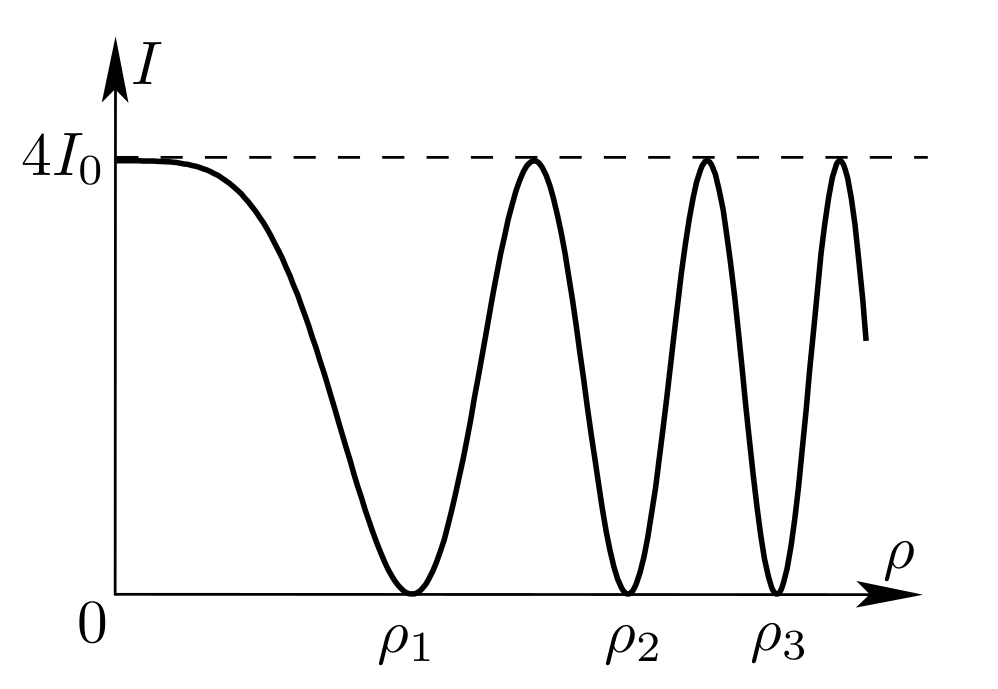
\includegraphics[width=\linewidth]{3.51.png}
    \caption{Зависимость $I(\rho)$}
    \label{img::3_51}
\end{wrapfigure}

Принимая начальную фазу на оси $z$ в плоскости $z = 0$ нулевой, запишем:
$\varphi = \frac{k}{2 z_0} \rho^2$. Мы полагаем, таким образом, что колебания опорной (плоской)
волны и сферической волны в точке $(x = 0,y = 0)$ синфазны. Тогда получим

\begin{equation}
    I(\rho) = 2 a^2 \left( 1 + \cos \frac{k \rho^2}{2 z_0} \right)
\end{equation}
\\
Мы видим, что интерференционная картина имеет вид колец, центр которых находится в начале координат. 
Функция $I(\rho)$ показана на рис. \ref{img::3_51}. Радиус первого (тёмного) кольца $\rho_1$
находим из условия $k \frac{\rho_1^2}{2 z_0} = \pi$ (при этом 
$\cos \left( k \frac{\rho_1^2}{2 z_0} \right)$ и $I(\rho_1) = 0$), откуда получаем: 
$\rho_1 = \sqrt{\lambda z_0}$. Вообще радиусы светлых и тёмных колец находятся по формуле

\begin{equation}
    \rho_m  = \sqrt{m \lambda z_0}
\end{equation}
\\
(при $m$ нечётном — тёмные кольца, при $m$ чётном — светлые), которая совпадает с выражением, 
определяющим радиусы тёмных и светлых колец в зонной пластинке Френеля.

Отличие состоит в том, что в нашем случае переход от светлых колец к тёмным происходит плавно. 
Интерференционная картина \eqref{eq::3.85} (голограмма точечного источника) показана на
рис. \ref{img::3_52} и называется зонной решёткой Габора. Как следует из проведённого выше анализа, 
\begin{wrapfigure}{r}{0.3\linewidth}
    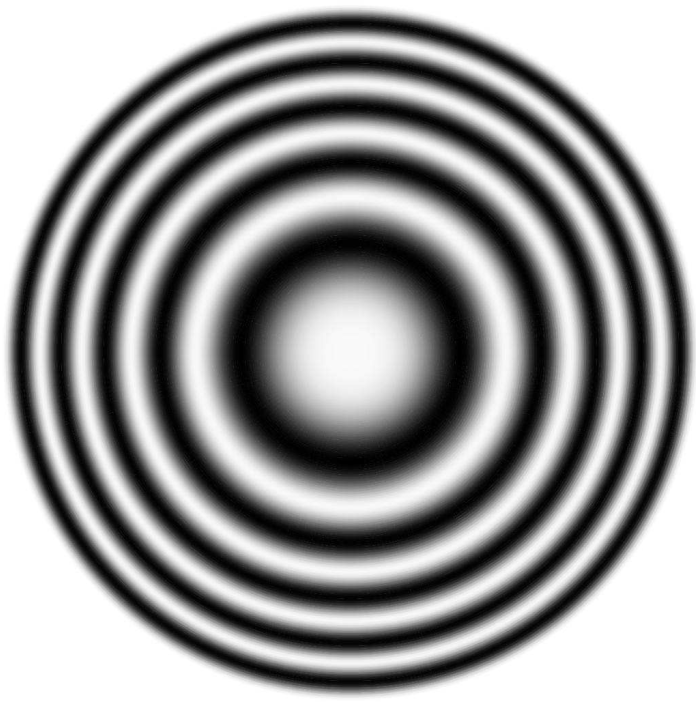
\includegraphics[width=\linewidth]{3.52.png}
    \caption{Зависимость $I(\rho)$}
    \label{img::3_52}
\end{wrapfigure}
зонная решётка Габора работает одновременно и как собирающая линза (фокусируя параллельный пучок 
света в точку $S''$ -- действительный фокус зонной пластинки), и как рассеивающая линза, которая 
преобразует параллельный пучок, падающий на пластинку, в расходящуюся сферическую волну, исходящую из
мнимого фокуса $S'$, и как плоскопараллельная пластинка, поскольку часть света за пластинкой 
сохраняет структуру освещающего параллельного пучка.